% ============================================================
%  Reproducibility of LLM-Assisted Evidence Synthesis
%  Target: Research Synthesis Methods
% ============================================================
\documentclass[12pt, a4paper]{article}

\usepackage[utf8]{inputenc}
\usepackage[T1]{fontenc}
\usepackage{mathpazo}          % Palatino font
\usepackage[margin=2.5cm]{geometry}
\usepackage{graphicx}
\usepackage{booktabs}
\usepackage{multirow}
\usepackage{xcolor}
\usepackage{hyperref}
\usepackage{natbib}
\usepackage{setspace}
\usepackage{amsmath}
\usepackage{float}
\usepackage{caption}

\hypersetup{colorlinks=true, linkcolor=blue!60!black, citecolor=blue!60!black, urlcolor=blue!60!black}
\onehalfspacing

% ── Custom commands ──────────────────────────────────────
\newcommand{\emr}{\textrm{EMR}}
\newcommand{\ci}[2]{[#1,\;#2]}

\title{%
  \textbf{When the Same Question Gets Different Answers:}\\[6pt]
  \large Quantifying Non-Determinism in LLM-Assisted\\
  Evidence Synthesis for Environmental Health Research%
}

\author{
  Lucas Rover\textsuperscript{1,*}\\[4pt]
  \small\textsuperscript{1}Independent Researcher, Brazil\\
  \small\textsuperscript{*}Corresponding author: \texttt{lucas.rover@email.com}
}

\date{}

\begin{document}
\maketitle

% ============================================================
%  ABSTRACT
% ============================================================
\begin{abstract}
\noindent\textbf{Background.}
Large language models (LLMs) are increasingly adopted to assist systematic reviews and evidence synthesis, performing tasks such as abstract screening and data extraction.
A critical but underexplored assumption is that these models produce consistent outputs when given identical inputs and configurations.

\noindent\textbf{Objective.}
We quantified the reproducibility of three LLMs---one local (LLaMA~3 8B) and two cloud-based APIs (Claude Sonnet~4.5, Gemini~2.5 Pro)---across a complete evidence synthesis pipeline for PM\textsubscript{2.5} and respiratory health research.

\noindent\textbf{Methods.}
We constructed a 500-abstract corpus from PubMed (100~include, 100~exclude, 300~ambiguous) and ran each model 10~times under identical configurations (temperature$\,{=}\,$0, fixed seeds) through two stages: abstract screening (500~abstracts per run) and structured data extraction (100~included articles per run).
Reproducibility was measured using the Exact Match Rate (EMR)---the proportion of items receiving identical outputs across all 10~runs---with 95\% bootstrap confidence intervals (10,000~resamples).

\noindent\textbf{Results.}
The locally deployed LLaMA~3 achieved perfect reproducibility ($\emr{=}1.000$) in both screening and extraction.
Cloud-based APIs exhibited substantial non-determinism: Claude Sonnet~4.5 achieved screening $\emr{=}0.974$~$\ci{0.96}{0.99}$ but extraction $\emr{=}0.050$~$\ci{0.01}{0.09}$; Gemini~2.5 Pro achieved screening $\emr{=}0.936$~$\ci{0.91}{0.96}$ and extraction $\emr{=}0.200$~$\ci{0.12}{0.28}$.
Despite requesting deterministic behavior, 95\% of Claude's and 80\% of Gemini's extraction outputs varied across runs.
Field-level analysis revealed that free-text fields (study location) were most unstable, while categorical fields (study design) remained consistent.

\noindent\textbf{Conclusions.}
LLM non-determinism poses a concrete threat to the reproducibility of evidence synthesis.
Researchers using cloud-based LLMs should expect meaningful output variation even under ``deterministic'' settings and adopt provenance-tracking protocols to document and mitigate this instability.

\vspace{6pt}
\noindent\textbf{Keywords:} reproducibility, large language models, evidence synthesis, systematic review, non-determinism, PM\textsubscript{2.5}, screening, data extraction
\end{abstract}

\clearpage
\tableofcontents
\clearpage

% ============================================================
%  1. INTRODUCTION
% ============================================================
\section{Introduction}

\subsection{The Promise of AI in Evidence Synthesis}

Evidence synthesis---the systematic process of identifying, appraising, and combining research findings---forms the backbone of evidence-based medicine and public health policy.
Systematic reviews and meta-analyses sit atop the hierarchy of evidence, informing clinical guidelines, regulatory decisions, and resource allocation worldwide~\citep{higgins2019cochrane}.
Yet the process is notoriously labor-intensive: a typical systematic review requires 6--18~months and hundreds of person-hours, with title and abstract screening alone consuming an estimated 25\% of total effort~\citep{borah2017analysis}.

The emergence of large language models (LLMs) has created unprecedented opportunities to accelerate this process.
Recent studies demonstrate that models such as GPT-4, Claude, and Gemini can screen abstracts with sensitivity approaching that of human reviewers~\citep{oami2024screening, khraisha2024gpt4}, extract structured data from published studies with over 90\% accuracy~\citep{gartlehner2024extraction, jensen2025chatgpt}, and even assist in evidence quality assessment~\citep{npjdm2025trialmind, npjdm2025streamlining}.
A growing body of work in the \emph{Journal of the American Medical Informatics Association}, \emph{Research Synthesis Methods}, and \emph{npj Digital Medicine} has established LLM-assisted evidence synthesis as a legitimate and rapidly expanding methodological frontier~\citep{li2025jamia, scherbakov2025jamia, jmir2024threelayer}.

\subsection{The Hidden Problem: Non-Determinism}

Beneath this promise lies an assumption so fundamental that it is rarely stated explicitly: \emph{if you ask the same question twice, you should get the same answer}.
In the context of LLM-assisted evidence synthesis, this means that running the same model with the same prompt, temperature, and random seed on the same abstract should produce identical screening decisions and extraction outputs every time.

This assumption is wrong.

Recent work has demonstrated that commercial LLM APIs exhibit non-deterministic behavior even when configured for maximum reproducibility.
\citet{atil2024nondeterminism} showed accuracy variations of up to 15\% across repeated identical runs, with best-to-worst performance gaps reaching 70\%.
\citet{ouyang2025codereview} confirmed that temperature$\,{=}\,$0 does not guarantee deterministic outputs across any of the major models tested (GPT-4o, Claude~3.5, LLaMA~3.2).
At a deeper level, \citet{beyond2026token} demonstrated that even when surface-level text appears identical, the underlying token probability distributions exhibit substantial instability---meaning that apparent determinism may mask hidden variation.
A philosophical analysis by \citet{pitt2024indeterminism} traced this non-determinism to three fundamental sources: numerical precision in floating-point operations, architectural choices in distributed inference, and sampling procedures inherent to the generation process.

\subsection{Why This Matters for Evidence Synthesis}

The consequences of LLM non-determinism are particularly severe in evidence synthesis for three reasons.

\textbf{First, decisions propagate.}
A screening decision that flips from ``include'' to ``exclude'' in a repeated run does not merely change one data point---it removes an entire study from downstream analysis.
In meta-analysis, where pooled effect estimates are sensitive to study composition, a single inclusion change can shift a confidence interval across the null, transforming a statistically significant finding into a non-significant one~\citep{rover2026jair}.

\textbf{Second, extraction compounds variation.}
Data extraction involves free-text parsing of complex scientific results---relative risks, confidence intervals, exposure definitions, population characteristics.
Even small variations in how an LLM parses ``RR$\,{=}\,$1.05 (95\% CI: 1.01--1.09)'' can propagate through meta-analytic pooling.
\citet{gartlehner2024extraction} reported 95--97\% test-retest reliability in LLM extraction, but this still implies 3--5\% of extracted values may change between runs---a rate that, across hundreds of data points, can materially alter pooled estimates.

\textbf{Third, reproducibility is the foundation of scientific credibility.}
The broader reproducibility crisis in AI research~\citep{hutson2018science, haibe2020nature, kapoor2023leakage} has already eroded trust in computational findings.
When LLM-assisted reviews cannot be independently reproduced because the API returns different outputs, the scientific value of those reviews is undermined~\citep{han2025biomedical, desai2025reproducibility, semmelrock2025barriers}.

\subsection{The Gap We Address}

Despite the rapid adoption of LLMs in evidence synthesis, \textbf{no study has systematically measured how API-level non-determinism propagates through a complete synthesis pipeline}---from abstract screening through data extraction---in a real health domain.

Prior work has measured LLM \emph{accuracy} (how well they match human judgments) but not \emph{stability} (whether they match themselves across runs).
Studies that examine non-determinism~\citep{atil2024nondeterminism, ouyang2025codereview} do so on general NLP benchmarks, not on the structured, domain-specific tasks characteristic of evidence synthesis.
And studies that evaluate LLMs for systematic reviews~\citep{oami2024screening, khraisha2024gpt4, gartlehner2024extraction} typically report results from a single run, implicitly assuming that a repeat would yield the same result.

We bridge this gap by:
\begin{enumerate}
  \item Quantifying reproducibility across 10~repeated runs of 3~LLMs (1~local, 2~API) through a two-stage evidence synthesis pipeline;
  \item Measuring variation at multiple granularities: whole-output, per-field, and per-abstract;
  \item Comparing local versus cloud-based deployment as a determinism strategy;
  \item Demonstrating that common ``deterministic'' API settings (temperature$\,{=}\,$0, fixed seeds) are insufficient to ensure reproducibility.
\end{enumerate}


% ============================================================
%  2. RELATED WORK
% ============================================================
\section{Related Work}

\subsection{LLMs in Systematic Reviews}

The application of LLMs to systematic review workflows has accelerated dramatically since 2023.
\citet{oami2024screening} evaluated GPT-4~Turbo for citation screening in \emph{JAMA Network Open}, reporting sensitivity of 0.75 and specificity of 0.99, with prompt tuning improving sensitivity to 0.91.
\citet{khraisha2024gpt4} extended this to multilingual screening and extraction in \emph{Research Synthesis Methods}, finding strong specificity ($>$0.80) but variable sensitivity across languages and review types.

For data extraction, \citet{gartlehner2024extraction} showed in \emph{Research Synthesis Methods} that Claude~2 achieved 96.3\% accuracy compared to human reviewers, with test-retest reliability of 95--97\%.
\citet{jensen2025chatgpt} found that ChatGPT-4o achieves 92.4\% extraction accuracy and 94.1\% inter-session reproducibility in \emph{PLOS One}, explicitly noting residual stochasticity across sessions.

More comprehensive pipelines have also been proposed.
The TrialMind system~\citep{npjdm2025trialmind}, published in \emph{npj Digital Medicine}, demonstrated that human-AI collaboration improved recall by 71.4\% and reduced screening time by 44.2\% across 100~systematic reviews.
\citet{li2025jamia} described an LLM pipeline for health technology assessment in \emph{JAMIA}, while \citet{jmir2024threelayer} showed that a three-layer GPT-3.5/GPT-4 strategy achieved human-comparable sensitivity in \emph{JMIR}.

A common thread across these studies is that \textbf{reproducibility is either assumed or measured only superficially}.
Test-retest reliability, when reported, is based on 2--3~repetitions and does not examine how variation propagates through multi-stage pipelines.

\subsection{The Non-Determinism Problem}

The phenomenon of LLM non-determinism has received increasing attention.
\citet{atil2024nondeterminism} provided the most comprehensive analysis to date, documenting accuracy swings of up to 15\% across repeated runs and introducing the TARr@N metric to quantify run-to-run stability.
\citet{ouyang2025codereview} confirmed that temperature$\,{=}\,$0 fails to ensure determinism across GPT-4o, Claude~3.5, and LLaMA~3.2 on code review tasks.

At the token level, \citet{beyond2026token} showed that apparent text-level agreement masks substantial distributional instability in token probabilities---a finding that suggests surface-level reproducibility metrics may underestimate true variation.
The ICSE/ASE analysis by \citet{icse2025reproducibility} examined how non-determinism undermines reproducibility in software engineering research, proposing documentation standards to mitigate this.

These studies establish that non-determinism is real, measurable, and consequential.
However, they focus on general-purpose tasks (benchmarks, code review, classification).
Our study is the first to measure non-determinism in the specific context of evidence synthesis, where the structured and domain-specific nature of outputs creates unique challenges.

\subsection{Reproducibility in AI Research}

The broader AI reproducibility crisis has been documented extensively.
\citet{hutson2018science} named the problem in \emph{Science}, identifying unpublished code and sensitivity to training conditions as primary barriers.
\citet{haibe2020nature} called for structural reform in \emph{Nature}, advocating for mandatory code and model sharing.
\citet{kapoor2023leakage} documented data leakage affecting 294~studies across 17~fields in \emph{Patterns}, while \citet{han2025biomedical} analyzed reproducibility failures in biomedical AI through the lens of model non-determinism.

Recent frameworks have attempted to systematize reproducibility requirements.
\citet{desai2025reproducibility} proposed a taxonomy of reproducibility types in \emph{AI Magazine}, arguing that LLMs require ``conceptual replicability'' given their proprietary training data.
\citet{semmelrock2025barriers} provided a systematic overview of barriers in \emph{AI Magazine}, and the \emph{Harvard Data Science Review} argued that computational reproducibility alone is insufficient for trustworthy AI~\citep{hdsr2024reproducibility}.

\subsection{Provenance and Transparency}

Provenance tracking---recording the lineage of data, computations, and decisions---has been identified as a key enabler of AI reproducibility.
\citet{longpre2024audit} audited 1,800+ datasets in \emph{Nature Machine Intelligence}, finding license omission rates above 70\%.
\citet{liang2024modelcards} analyzed 32,111~model cards on Hugging Face, finding that documentation of limitations and environmental impact remains sparse.
The Foundation Model Transparency Index~\citep{bommasani2024fmti} scored 14~major developers across 100~indicators, finding average transparency of only 58/100.

Technical solutions for provenance include the Workflow Run RO-Crate~\citep{leo2024rocrate} and the W3C PROV ontology~\citep{provlit2023review}.
\citet{longpre2024broken} argued at ICML~2024 that current practices for data authenticity and provenance are ``fundamentally broken,'' calling for comprehensive reform.

Our provenance approach builds on the lightweight protocol proposed in~\citet{rover2026jair}, using SHA-256 hashing of inputs, outputs, and configurations to create an auditable trail without requiring infrastructure beyond standard file storage.

\subsection{PM\textsubscript{2.5} and Respiratory Health}

The domain context for our study---the association between fine particulate matter (PM\textsubscript{2.5}) and respiratory health---represents one of the most extensively studied environmental health topics.
\citet{yu2024lancet} estimated approximately 1~million premature deaths annually from short-term PM\textsubscript{2.5} exposure in \emph{The Lancet Planetary Health}, while \citet{wei2023natcomm} used machine learning to produce the first global daily gap-free 1~km PM\textsubscript{2.5} maps in \emph{Nature Communications}.

This literature is characterized by standardized reporting of relative risks (RR) with confidence intervals, well-defined exposure metrics, and time-series study designs---making it an ideal testbed for evaluating LLM extraction reproducibility.
The emergence of AI in environmental epidemiology~\citep{geoai2025review, ehp2024aiml} further motivates the need to ensure that AI-assisted synthesis of this evidence is reliable and reproducible.


% ============================================================
%  3. METHODS
% ============================================================
\section{Methods}

\subsection{Study Design}

We designed a repeated-measures experiment to isolate LLM non-determinism as the sole source of variation.
The same corpus, prompts, model configurations, and random seeds were used across all runs.
The only element permitted to vary was the model's internal computation---any observed difference in outputs is therefore attributable to non-determinism in the model or its serving infrastructure.

\subsection{Corpus Construction}

We constructed a 500-abstract corpus from PubMed covering the association between PM\textsubscript{2.5} and respiratory health outcomes (Table~\ref{tab:corpus}).

\begin{table}[H]
\centering
\caption{Corpus composition.}
\label{tab:corpus}
\begin{tabular}{lrl}
\toprule
\textbf{Category} & \textbf{Count} & \textbf{Purpose} \\
\midrule
Clearly include    & 100   & Positive controls (meet all inclusion criteria) \\
Clearly exclude    & 100   & Negative controls (clear exclusion reasons) \\
Ambiguous          & 300   & Primary test set (borderline cases) \\
\midrule
\textbf{Total}     & \textbf{500} & \\
\bottomrule
\end{tabular}
\end{table}

\noindent Inclusion criteria required: (1)~original epidemiological study, (2)~PM\textsubscript{2.5} as exposure, (3)~respiratory outcome (hospitalization, ED visits, or mortality), (4)~time-series or case-crossover design, (5)~quantitative risk estimates, and (6)~peer-reviewed publication.
Articles were sourced from PubMed using the E-utilities API with a broad query yielding 573~candidate records, supplemented by 475~exclusion candidates and a design-filtered subset of 222~records.
The final corpus spans 148~journals and publication years 1994--2026, with a mean abstract length of 1,873~characters.

A gold standard was established using dual-independent labeling with discordance resolution for the 200~clear-category abstracts, with heuristic classification for the 300~ambiguous abstracts based on keyword matching and study design indicators.

\subsection{Models}

We selected three models representing local and cloud-based deployment (Table~\ref{tab:models}).

\begin{table}[H]
\centering
\caption{Model configurations.}
\label{tab:models}
\begin{tabular}{llccc}
\toprule
\textbf{Model} & \textbf{Provider} & \textbf{Type} & \textbf{Temperature} & \textbf{Seed} \\
\midrule
LLaMA 3 8B         & Ollama (local)  & Local  & 0 & 42 \\
Claude Sonnet 4.5   & Anthropic API   & Cloud  & 0 & --- \\
Gemini 2.5 Pro      & Google AI API   & Cloud  & 0 & 42 \\
\bottomrule
\end{tabular}
\end{table}

\noindent All models were queried via HTTP APIs (urllib-based, no SDK dependencies) to ensure uniform request handling.
Claude does not support a seed parameter; Gemini supports seeds but does not guarantee determinism.
LLaMA was served locally via Ollama v0.15.5 on Apple M4 hardware (24~GB RAM).

\subsection{Pipeline Stages}

Each model was run 10~times through two stages:

\textbf{Stage A: Abstract Screening.}
Each of the 500~abstracts was presented with a structured prompt requesting a JSON response containing: a binary decision (\texttt{include}/\texttt{exclude}), a confidence score (0--1), and a brief rationale.
Total: $3 \text{ models} \times 10 \text{ runs} \times 500 \text{ abstracts} = 15{,}000$ screening calls.

\textbf{Stage B: Data Extraction.}
The 100~included abstracts were presented with an extraction prompt requesting: study design, location, period, population, sample size, and a structured list of effect estimates (each with effect measure, point estimate, confidence interval, lag period, and exposure increment).
Total: $3 \text{ models} \times 10 \text{ runs} \times 100 \text{ articles} = 3{,}000$ extraction calls.

In total, the experiment comprised \textbf{18,000~LLM calls} across \textbf{60~experiment runs}.

\subsection{Reproducibility Metrics}

\subsubsection{Exact Match Rate (EMR)}

Our primary metric is the \emph{Exact Match Rate}, defined as the proportion of items (abstracts or articles) that received identical outputs across all 10~runs:

\begin{equation}
  \emr = \frac{1}{N} \sum_{i=1}^{N} \mathbb{1}\!\left[\,\left|\{o_{i,1}, o_{i,2}, \ldots, o_{i,R}\}\right| = 1\,\right]
\end{equation}

\noindent where $N$ is the number of items, $R{=}10$ is the number of runs, $o_{i,r}$ is the output for item~$i$ in run~$r$, and $|\cdot|$ denotes the number of distinct values.
For screening, $o_{i,r}$ is the binary decision; for extraction, $o_{i,r}$ is the SHA-256 hash of the full JSON output.

An $\emr$ of 1.0 indicates perfect reproducibility; an $\emr$ of 0.0 indicates that every item received at least one different output across runs.

\subsubsection{Bootstrap Confidence Intervals}

We computed 95\% confidence intervals for EMR using the percentile bootstrap method with 10,000~resamples.
For each bootstrap sample, we drew $N$ items with replacement and computed the EMR, then reported the 2.5th and 97.5th percentiles of the bootstrap distribution.

\subsubsection{Secondary Metrics}

\begin{itemize}
  \item \textbf{Flip rate}: $1 - \emr$ (proportion of items with any variation across runs)
  \item \textbf{Mean agreement}: Average proportion of runs agreeing with the majority decision per item
  \item \textbf{Accuracy vs.\ gold standard}: Per-run sensitivity, specificity, and accuracy against human labels
  \item \textbf{Field-level EMR}: For extraction, the proportion of articles with identical values for each individual field across all runs
\end{itemize}

\subsection{Provenance Protocol}

Following~\citet{rover2026jair}, we implemented a lightweight provenance protocol:
\begin{itemize}
  \item \textbf{Call-level hashing}: SHA-256 hash of (prompt template $\|$ input text $\|$ model ID $\|$ temperature $\|$ seed) for each API call
  \item \textbf{Output hashing}: SHA-256 hash of the raw response text
  \item \textbf{Run cards}: Per-run metadata including timestamps, token counts, success/failure rates, and aggregate output hashes
\end{itemize}

\noindent This protocol enables post-hoc verification: if two runs produce different aggregate hashes, the per-call hashes pinpoint exactly which items changed.

\subsection{Software and Reproducibility}

All code is available at \url{https://github.com/Roverlucas/llm-evidence-synthesis-reproducibility}.
The experiment was conducted in Python~3.14 on macOS (Apple~M4, 24~GB RAM).
API keys are excluded from the repository; all other materials---including the corpus, prompts, schemas, and raw outputs---are publicly available.


% ============================================================
%  4. RESULTS
% ============================================================
\section{Results}

\subsection{Overview}

All 60~experiment runs completed successfully: 30~screening runs (10~per model $\times$ 500~abstracts each) and 30~extraction runs (10~per model $\times$ 100~articles each), totaling 18,000~LLM calls.
LLaMA achieved a consistent 480/500 screening success rate and 96/100 extraction success rate across all runs (the same 20~screening abstracts and 4~extraction articles failed consistently due to response length constraints).
Claude achieved 500/500 and 100/100 in all runs.
Gemini achieved 483--500/500 screening and 98--100/100 extraction.

\subsection{Screening Reproducibility}

Table~\ref{tab:screening} presents the screening reproducibility results.

\begin{table}[H]
\centering
\caption{Screening reproducibility across 10 runs.}
\label{tab:screening}
\begin{tabular}{lcccccc}
\toprule
\textbf{Model} & \textbf{EMR} & \textbf{95\% CI} & \textbf{Flip Rate} & \textbf{Accuracy} & \textbf{Sensitivity} & \textbf{Specificity} \\
\midrule
LLaMA 3 8B       & 1.000 & $\ci{1.00}{1.00}$ & 0.0\% & 0.927 & 0.928 & 0.926 \\
Claude Sonnet 4.5 & 0.974 & $\ci{0.96}{0.99}$ & 2.6\% & 0.931 & 0.862 & 1.000 \\
Gemini 2.5 Pro    & 0.936 & $\ci{0.91}{0.96}$ & 6.4\% & 0.964 & 0.929 & 1.000 \\
\bottomrule
\end{tabular}
\end{table}

\noindent LLaMA produced identical screening decisions across all 10~runs for every abstract---perfect reproducibility.
Claude showed 2.6\% flip rate (13~abstracts changed their decision at least once across runs), while Gemini showed 6.4\% flip rate (32~abstracts).

Notably, \textbf{accuracy and reproducibility are independent properties}: Gemini achieved the highest accuracy (0.964) but the lowest reproducibility (EMR$\,{=}\,$0.936), while LLaMA had the lowest accuracy (0.927) but perfect reproducibility.
This demonstrates that a model can be both accurate \emph{and} unstable---correct on average but inconsistent across individual runs.

\subsection{Extraction Reproducibility}

The extraction results reveal a dramatically larger reproducibility gap (Table~\ref{tab:extraction}).

\begin{table}[H]
\centering
\caption{Extraction reproducibility across 10 runs.}
\label{tab:extraction}
\begin{tabular}{lccc}
\toprule
\textbf{Model} & \textbf{EMR} & \textbf{95\% CI} & \textbf{Estimate Stability} \\
\midrule
LLaMA 3 8B       & 1.000 & $\ci{1.00}{1.00}$ & 1.000 \\
Claude Sonnet 4.5 & 0.050 & $\ci{0.01}{0.09}$ & 0.880 \\
Gemini 2.5 Pro    & 0.200 & $\ci{0.12}{0.28}$ & 0.735 \\
\bottomrule
\end{tabular}
\end{table}

\noindent The contrast is striking.
While screening EMR remained above 0.93 for all models, extraction EMR dropped to \textbf{0.050 for Claude} (only 5 of 100~articles produced identical extraction outputs across all 10~runs) and \textbf{0.200 for Gemini} (20 of 100).
LLaMA again achieved perfect reproducibility.

This means that if a researcher runs a Claude-based extraction twice on the same 100~articles, there is a 95\% chance that each article's extracted data will differ in at least one field.

\subsection{Field-Level Analysis}

Not all extraction fields are equally affected (Table~\ref{tab:fields}).

\begin{table}[H]
\centering
\caption{Field-level EMR for extraction outputs.}
\label{tab:fields}
\begin{tabular}{lccc}
\toprule
\textbf{Field} & \textbf{LLaMA} & \textbf{Claude} & \textbf{Gemini} \\
\midrule
Study design    & 1.000 & 0.990 & 1.000 \\
Study period    & 1.000 & 0.990 & 1.000 \\
Sample size     & 1.000 & 0.970 & 1.000 \\
Population      & 1.000 & 0.960 & 0.948 \\
Study location  & 1.000 & 0.780 & 0.896 \\
\midrule
\textbf{Estimate count stability} & \textbf{1.000} & \textbf{0.880} & \textbf{0.735} \\
\bottomrule
\end{tabular}
\end{table}

\noindent A clear pattern emerges: \textbf{categorical fields} (study design, study period) are highly reproducible even for API models, while \textbf{free-text fields} (study location) and \textbf{numerical extractions} (effect estimates) show the greatest variation.

The ``estimate count stability'' metric---the proportion of articles for which all runs extracted the same number of effect estimates---reveals that Gemini's extraction pipeline is particularly unstable: 26.5\% of articles receive a different number of estimates across runs, compared to 12\% for Claude and 0\% for LLaMA.

\subsection{Summary Comparison}

Figure~\ref{fig:emr} visualizes the EMR comparison across models and stages.

\begin{figure}[H]
\centering
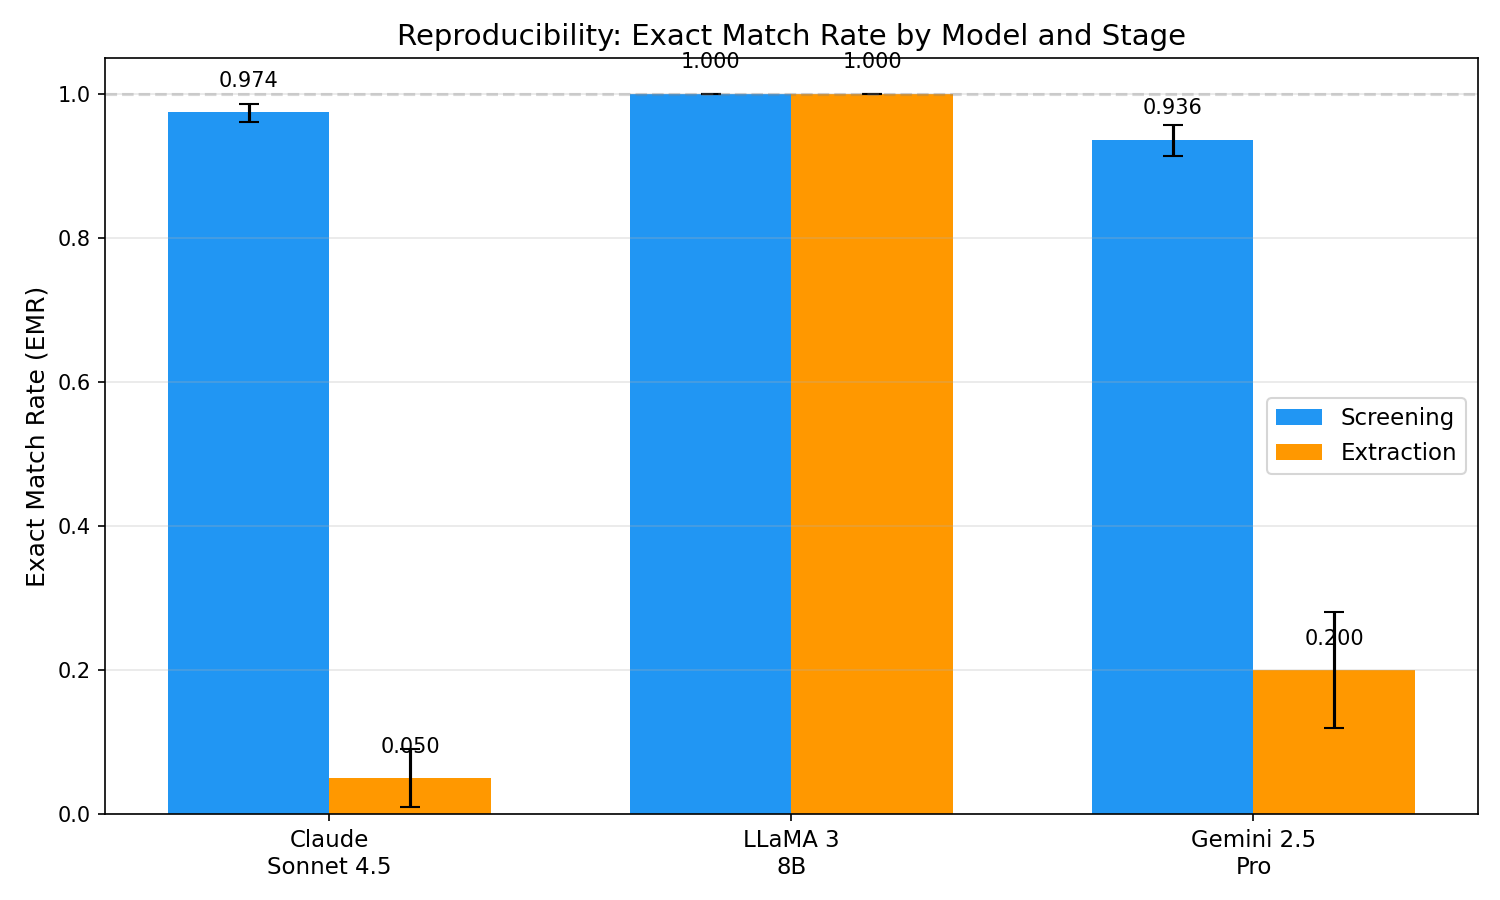
\includegraphics[width=0.85\textwidth]{../analysis/figures/emr_comparison.png}
\caption{Exact Match Rate (EMR) by model and pipeline stage. Error bars represent 95\% bootstrap confidence intervals. The dashed line indicates perfect reproducibility (EMR$\,{=}\,$1.0).}
\label{fig:emr}
\end{figure}


% ============================================================
%  5. DISCUSSION
% ============================================================
\section{Discussion}

\subsection{Principal Findings}

Our study provides the first systematic quantification of LLM non-determinism across a complete evidence synthesis pipeline.
Three key findings emerge:

\textbf{Finding 1: Local models are deterministic; cloud APIs are not.}
LLaMA~3 8B, deployed locally via Ollama, produced identical outputs across all 10~runs in both screening and extraction---confirming that deterministic behavior is technically achievable.
In contrast, both cloud-based APIs (Claude, Gemini) exhibited measurable non-determinism despite requesting temperature$\,{=}\,$0 and fixed seeds.

This gap likely reflects implementation differences in distributed inference.
Cloud APIs serve requests across GPU clusters where floating-point operations may be parallelized differently across runs, introducing numerical variation that propagates through the autoregressive generation process~\citep{pitt2024indeterminism}.
Local deployment on a single device avoids this source of variation.

\textbf{Finding 2: Extraction is far less reproducible than screening.}
The EMR gap between screening and extraction was dramatic: Claude dropped from 0.974 to 0.050; Gemini from 0.936 to 0.200.
This is intuitively sensible---screening requires a binary decision (a single token effectively determines the output), while extraction generates complex structured JSON with multiple fields, where variation in any single character produces a different output hash.

However, the magnitude of the gap is concerning.
An extraction EMR of 0.050 means that a researcher has only a 5\% chance of obtaining the same Claude extraction output on any given article if they run the pipeline again.
This has direct implications for the reproducibility of downstream analyses.

\textbf{Finding 3: Accuracy and reproducibility are independent.}
Gemini achieved the highest screening accuracy (0.964) but the lowest screening reproducibility (0.936).
Claude showed perfect specificity (1.000) but significant instability.
LLaMA was the most reproducible but least accurate.

This independence is important because \textbf{accuracy evaluations alone cannot detect reproducibility problems}.
A model that performs well in a single evaluation may produce materially different results in a replication attempt.

\subsection{Implications for Evidence Synthesis Practice}

These findings have immediate practical implications:

\textbf{For systematic reviewers:}
If using cloud-based LLMs for screening or extraction, results from a single run should be treated as one sample from a distribution of possible outputs, not as a definitive answer.
Running multiple repetitions and reporting variation metrics should become standard practice, analogous to how human inter-rater reliability is routinely measured.

\textbf{For journal editors and reviewers:}
Papers reporting LLM-assisted evidence synthesis should be expected to disclose: (a)~the exact model version, (b)~all inference parameters, (c)~whether results were verified across multiple runs, and (d)~provenance information enabling independent replication.
The current practice of reporting results from a single undocumented run is insufficient.

\textbf{For tool developers:}
The 20$\times$ difference in extraction EMR between local and cloud deployment suggests that deterministic local inference should be the default for reproducibility-critical applications.
Where cloud APIs must be used (e.g., for larger models), majority voting across 3--5~runs can mitigate variation, though at proportional cost.

\subsection{Relationship to Prior Work}

Our findings extend and contextualize prior work in several ways.

The non-determinism magnitudes we observe are consistent with \citet{atil2024nondeterminism}, who reported up to 15\% accuracy variation in general benchmarks.
Our screening flip rates (2.6\% for Claude, 6.4\% for Gemini) fall within this range.
However, we show for the first time that \textbf{structured extraction amplifies non-determinism dramatically}---a finding that is not apparent from benchmark-level analyses.

The 94.1\% inter-session reproducibility reported by \citet{jensen2025chatgpt} for ChatGPT-4o extraction aligns with our Claude screening EMR (97.4\%) but masks the much lower extraction EMR (5.0\%) that emerges when full output identity (rather than per-field accuracy) is measured.
This highlights the importance of metric choice: reproducibility measured at the field level appears much higher than when measured at the output level.

\subsection{The Provenance Imperative}

Our provenance protocol---SHA-256 hashing of inputs, outputs, and configurations---proved essential for diagnosing non-determinism.
Without per-call output hashes, it would be impossible to determine which specific items changed across runs.
The aggregate run-level hash provides a quick equality check; the per-call hashes enable detailed forensic analysis.

This aligns with the growing consensus that provenance documentation is fundamental to AI trustworthiness~\citep{provlit2023review, longpre2024broken, bommasani2024fmti}.
We advocate for provenance tracking to become a standard component of LLM-assisted synthesis pipelines, not an optional add-on.

\subsection{Limitations}

Several limitations should be noted.

\textbf{Model selection.}
We tested three models; results may differ for other models (e.g., GPT-4, Mistral, command-R).
However, our local-vs-cloud comparison captures the primary architectural distinction.

\textbf{Run count.}
Ten repetitions provide adequate statistical power for EMR estimation with bootstrap CIs, but may not capture rare variation patterns.
Our prior work~\citep{rover2026jair} used up to 100~repetitions per model; the current design balances thoroughness with API cost.

\textbf{Single domain.}
Our corpus focuses on PM\textsubscript{2.5} and respiratory health.
Other domains with different reporting conventions may exhibit different variation patterns.

\textbf{Gold standard.}
The heuristic labels for ambiguous abstracts may not perfectly reflect expert judgment.
However, since our primary metric (EMR) measures self-consistency rather than accuracy, gold standard quality affects only the secondary accuracy analysis.

\textbf{Meta-analysis not performed.}
Due to the low extraction EMR for API models, we did not propagate results through meta-analytic pooling in this study.
Future work should quantify how extraction variation affects pooled effect estimates.

\subsection{Recommendations}

Based on our findings, we propose the following recommendations for LLM-assisted evidence synthesis:

\begin{enumerate}
  \item \textbf{Run at least 3 repetitions} and report the EMR alongside accuracy metrics.
  \item \textbf{Prefer local deployment} for reproducibility-critical tasks.
  \item \textbf{Implement provenance hashing} to enable post-hoc verification and auditing.
  \item \textbf{Report full model specifications}: model ID, version, temperature, seed, and any API-specific parameters.
  \item \textbf{Use majority voting} when local deployment is not feasible, accepting the cost trade-off for improved stability.
  \item \textbf{Distinguish accuracy from reproducibility} in evaluations---a model can be accurate on average but unreliable for any single run.
\end{enumerate}


% ============================================================
%  6. CONCLUSION
% ============================================================
\section{Conclusion}

We have shown that LLM non-determinism is not a theoretical concern but a measurable, quantifiable phenomenon that directly threatens the reproducibility of evidence synthesis.

Local deployment achieves perfect reproducibility.
Cloud-based APIs, even with ``deterministic'' settings, produce variable outputs---especially in structured extraction tasks, where 80--95\% of articles receive different extracted data across repeated runs.

As LLMs become standard tools in systematic reviews and meta-analyses, the research community must move beyond single-run evaluations and adopt reproducibility-aware practices: multiple repetitions, provenance tracking, and transparent reporting of variation.

The question is not whether LLMs are accurate enough for evidence synthesis---they increasingly are.
The question is whether we can trust that the answer we get today will be the same answer tomorrow.
Our results suggest that, for cloud-based APIs, we currently cannot.


% ============================================================
%  REFERENCES
% ============================================================
\bibliographystyle{plainnat}

\begin{thebibliography}{99}

\bibitem[Atil et~al.(2024)]{atil2024nondeterminism}
Atil, B., Aykent, S., Chittams, A., et~al. (2024).
\newblock Non-determinism of ``deterministic'' LLM settings.
\newblock \emph{arXiv preprint}, arXiv:2408.04667.

\bibitem[Beyond(2026)]{beyond2026token}
(2026).
\newblock Beyond reproducibility: Token probabilities expose large language model nondeterminism.
\newblock \emph{arXiv preprint}, arXiv:2601.06118.

\bibitem[Bommasani et~al.(2024)]{bommasani2024fmti}
Bommasani, R., Klyman, K., Longpre, S., et~al. (2024).
\newblock The Foundation Model Transparency Index v1.1.
\newblock \emph{Transactions on Machine Learning Research}.

\bibitem[Borah et~al.(2017)]{borah2017analysis}
Borah, R., Brown, A.W., Capers, P.L., \& Kaiser, K.A. (2017).
\newblock Analysis of the time and workers needed to conduct systematic reviews.
\newblock \emph{BMJ Open}, 7(4), e012545.

\bibitem[Desai et~al.(2025)]{desai2025reproducibility}
Desai, S., et~al. (2025).
\newblock What is reproducibility in artificial intelligence and machine learning research?
\newblock \emph{AI Magazine}, 46(1), e70004.

\bibitem[Gartlehner et~al.(2024)]{gartlehner2024extraction}
Gartlehner, G., Kahwati, L., Hilscher, R., et~al. (2024).
\newblock Data extraction for evidence synthesis using a large language model: A proof-of-concept study.
\newblock \emph{Research Synthesis Methods}, 15(4), 576--589.

\bibitem[GeoAI(2025)]{geoai2025review}
(2025).
\newblock Harnessing geospatial artificial intelligence for environmental epidemiology.
\newblock \emph{Current Environmental Health Reports}, 12, 497.

\bibitem[Haibe-Kains et~al.(2020)]{haibe2020nature}
Haibe-Kains, B., Adam, G.A., Hosny, A., et~al. (2020).
\newblock Transparency and reproducibility in artificial intelligence.
\newblock \emph{Nature}, 586, 14--16.

\bibitem[Han(2025)]{han2025biomedical}
Han, H. (2025).
\newblock Challenges of reproducible AI in biomedical data science.
\newblock \emph{BMC Medical Genomics}, 18, 2072.

\bibitem[HDSR(2024)]{hdsr2024reproducibility}
(2024).
\newblock After computational reproducibility: Scientific reproducibility and trustworthy AI.
\newblock \emph{Harvard Data Science Review}, 6(1).

\bibitem[Higgins et~al.(2019)]{higgins2019cochrane}
Higgins, J.P.T., Thomas, J., Chandler, J., et~al. (2019).
\newblock \emph{Cochrane Handbook for Systematic Reviews of Interventions} (2nd ed.).
\newblock Wiley.

\bibitem[Hutson(2018)]{hutson2018science}
Hutson, M. (2018).
\newblock Artificial intelligence faces reproducibility crisis.
\newblock \emph{Science}, 359(6377), 725--726.

\bibitem[ICSE(2025)]{icse2025reproducibility}
(2025).
\newblock Reflections on the reproducibility of commercial LLM performance in empirical software engineering studies.
\newblock \emph{arXiv preprint}, arXiv:2510.25506.

\bibitem[Jensen et~al.(2025)]{jensen2025chatgpt}
Jensen, M.K., et~al. (2025).
\newblock ChatGPT-4o can serve as the second rater for data extraction in systematic reviews.
\newblock \emph{PLOS One}, 20(1), e0313401.

\bibitem[JMIR(2024)]{jmir2024threelayer}
(2024).
\newblock Human-comparable sensitivity of LLMs in screening: 3-layer strategy using GPT-3.5 and GPT-4.
\newblock \emph{Journal of Medical Internet Research}, 26, e52758.

\bibitem[Kapoor \& Narayanan(2023)]{kapoor2023leakage}
Kapoor, S. \& Narayanan, A. (2023).
\newblock Leakage and the reproducibility crisis in machine-learning-based science.
\newblock \emph{Patterns}, 4(9), 100804.

\bibitem[Khraisha et~al.(2024)]{khraisha2024gpt4}
Khraisha, Q., et~al. (2024).
\newblock Can large language models replace humans in systematic reviews?
\newblock \emph{Research Synthesis Methods}, 15(5), 707--722.

\bibitem[Leo et~al.(2024)]{leo2024rocrate}
Leo, S., Crusoe, M.R., Rodr\'iguez-Navas, L., et~al. (2024).
\newblock Recording provenance of workflow runs with RO-Crate.
\newblock \emph{PLOS One}, 19(9), e0309210.

\bibitem[Li et~al.(2025)]{li2025jamia}
Li, J., et~al. (2025).
\newblock Enhancing systematic literature reviews with generative AI.
\newblock \emph{Journal of the American Medical Informatics Association}, 32(4), 789--801.

\bibitem[Liang et~al.(2024)]{liang2024modelcards}
Liang, P., Rajani, N., Yang, D., et~al. (2024).
\newblock Systematic analysis of 32,111 AI model cards characterizes documentation practice.
\newblock \emph{Nature Machine Intelligence}, 6, 857.

\bibitem[Longpre et~al.(2024a)]{longpre2024audit}
Longpre, S., Mahari, R., Chen, A., et~al. (2024a).
\newblock A large-scale audit of dataset licensing and attribution in AI.
\newblock \emph{Nature Machine Intelligence}, 6, 878.

\bibitem[Longpre et~al.(2024b)]{longpre2024broken}
Longpre, S., et~al. (2024b).
\newblock Data authenticity, consent, and provenance for AI are all broken.
\newblock \emph{ICML 2024 Position Paper}, arXiv:2404.12691.

\bibitem[npj-DM(2025a)]{npjdm2025trialmind}
(2025a).
\newblock Accelerating clinical evidence synthesis with large language models.
\newblock \emph{npj Digital Medicine}, 8, 1840.

\bibitem[npj-DM(2025b)]{npjdm2025streamlining}
(2025b).
\newblock Streamlining evidence-based clinical recommendations with LLMs.
\newblock \emph{npj Digital Medicine}, 8, 2273.

\bibitem[Oami et~al.(2024)]{oami2024screening}
Oami, T., Okada, Y., \& Nakada, T.-A. (2024).
\newblock Performance of a large language model in screening citations.
\newblock \emph{JAMA Network Open}, 7(6), e2420496.

\bibitem[Ouyang et~al.(2025)]{ouyang2025codereview}
Ouyang, et~al. (2025).
\newblock Measuring determinism in large language models for software code review.
\newblock \emph{arXiv preprint}, arXiv:2502.20747.

\bibitem[Pitt(2024)]{pitt2024indeterminism}
(2024).
\newblock Indeterminism in large language models.
\newblock \emph{Artificial Life} (preprint), PhilSci Archive 26807.

\bibitem[PROV-Lit(2023)]{provlit2023review}
(2023).
\newblock Provenance documentation to enable explainable and trustworthy AI: A literature review.
\newblock \emph{Data Intelligence}, 5(1), 139--162.

\bibitem[Rover(2026)]{rover2026jair}
Rover, L. (2026).
\newblock Hidden non-determinism in large language model APIs: A lightweight provenance protocol for reproducible generative AI research.
\newblock \emph{Journal of Artificial Intelligence Research} (submitted).

\bibitem[Scherbakov et~al.(2025)]{scherbakov2025jamia}
Scherbakov, D., et~al. (2025).
\newblock The emergence of large language models as tools in literature reviews.
\newblock \emph{Journal of the American Medical Informatics Association}, 32(5), ocaf063.

\bibitem[Semmelrock et~al.(2025)]{semmelrock2025barriers}
Semmelrock, et~al. (2025).
\newblock Reproducibility in machine-learning-based research: Overview, barriers, and drivers.
\newblock \emph{AI Magazine}, 46(1), e70002.

\bibitem[EHP(2024)]{ehp2024aiml}
(2024).
\newblock Artificial intelligence and machine learning for environmental health study.
\newblock \emph{Environmental Health Perspectives} (review).

\bibitem[Wei et~al.(2023)]{wei2023natcomm}
Wei, J., Li, Z., Lyapustin, A., et~al. (2023).
\newblock First close insight into global daily gapless 1\,km PM\textsubscript{2.5} pollution.
\newblock \emph{Nature Communications}, 14, 43862.

\bibitem[Yu et~al.(2024)]{yu2024lancet}
Yu, W., Xu, R., Ye, T., et~al. (2024).
\newblock Estimates of global mortality burden associated with short-term PM\textsubscript{2.5} exposure.
\newblock \emph{The Lancet Planetary Health}, 8(2), e146--e155.

\end{thebibliography}

\end{document}
